\section{Resultados}
\label{sec:4}

\subsection{Sección 1 de Resultados}
\label{sec:4.1}

El texto del artículo tiene interlineado sencillo; 12 puntos de tamaño de fuente; tipo de letra Times New Roman; las páginas están numeradas; se utiliza cursiva para las palabras en inglés en lugar de subrayado (excepto en las direcciones URL); y todas las ilustraciones, ecuaciones, figuras y tablas se encuentran enumeradas y colocadas en los lugares del texto apropiados, en vez de al final.
Además, se pueden incluir secciones para agrupar resultados, por ejemplo, según escenarios o método a usar.
Los resultados se pueden ver en tablas o ilustraciones, las cuales pueden complementar la explicación del texto (ver Ilustración \ref{fig1}).

\begin{figure}[h]
    \centering
    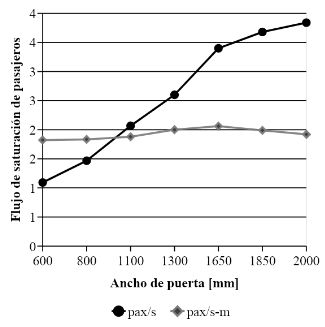
\includegraphics[width=0.5\textwidth]{imagenes/fig1.png}
    \caption{Flujo de saturación de pasajeros en función del ancho de puertas}\label{fig1}
\end{figure}
